\documentclass[aspectratio=169]{beamer}

\usepackage[croatian]{babel}
\usepackage[T1]{fontenc}
\usepackage[utf8]{inputenc}
\usepackage{lmodern}
\usepackage{microtype}
\usepackage{csquotes}
\usepackage[natbibapa]{apacite}
\usepackage{url}
\usepackage{fontawesome}

%%%%% titlepage
\title[]{\textit{Megastudy} paradigma i procesiranje jezika}
\subtitle{\footnotesize Izlaganje za Znanstveni kolokvij}
\author[]{Denis Vlašiček \\[5em]
    \scriptsize
    \url{https://osf.io/zqa7y/}
}
\date[]{\footnotesize \today}
%%%%%

%%%%% prilagodba referenci na hrvatski
\renewcommand{\BCBT}{}
\renewcommand{\BCBL}{}%  comma before last author when no. of authors > 2
\renewcommand{\BOthers}[1]{i sur.\hbox{}}% ``and others''
\renewcommand{\BBAA}{i}
\renewcommand{\BBAB}{i}
\renewcommand{\BIn}{U:}
\renewcommand{\BED}{Ur.\hbox{}}
\renewcommand{\BEDS}{Ur.\hbox{}}
\renewcommand{\BPGS}{str.\hbox{}}
\renewcommand{\BRetrievedFrom}{Preuzeto s:\hbox{}}
\renewcommand{\BEd}{izdanje}
\renewcommand{\BVOL}{svezak}
%%%%%

%%%%% beamer tema
\usetheme{CambridgeUS}

\usecolortheme{dove}

\setbeamertemplate{itemize items}[default]

\setbeamertemplate{itemize item}{\textbullet}
\setbeamertemplate{itemize subitem}{\(\triangleright\)}

\setbeamertemplate{section page}{
    \begin{centering}
        \Large
        \insertsection\par
    \end{centering}
}

\setbeameroption{hide notes}
%\setbeameroption{show only notes}
%\usepackage{pgfpages}
%\setbeameroption{show notes on second screen=left}

%%%%%

%%%%% serif font kao default
\usefonttheme{serif}
%%%%%

\setbeamertemplate{navigation symbols}{}

\makeatletter
\newenvironment{noheadline}{
    \setbeamertemplate{headline}{}
    \addtobeamertemplate{frametitle}{\vspace*{-0.9\baselineskip}}{}
}{}
\makeatother
%%%%%

%%%%% nastavljanje enumerate
\newcounter{saveenumi}
\newcommand{\seti}{\setcounter{saveenumi}{\value{enumi}}}
\newcommand{\conti}{\setcounter{enumi}{\value{saveenumi}}}

\resetcounteronoverlays{saveenumi}
%%%%%

%%%%5 fontsize za bibliografiju
\renewcommand*{\bibfont}{\scriptsize}
%%%%%

%%%%% tiny citep
\newcommand{\tinycitep}[1]{%
    \bgroup
    \scriptsize
    \citep{#1}
    \egroup}
%%%%%

\begin{document}

\begin{frame}
    \titlepage
\end{frame}

\section{\textit{Megastudy} paradigma}

\begin{noheadline}

\begin{frame}
    \sectionpage
\end{frame}

\end{noheadline}

\subsection{Uvod}

\begin{frame}
    \frametitle{Uvod}

    \begin{itemize}
        \item tradicionalni način ispitivanja --- faktorijalni eksperimenti

        \note[item]{klasični oblik ispitivanja u eksperimentalnoj kognitivnoj
            psihologiji}

        \note[item]{primjerice, ispitivanje frekvencije --- česte i rijetke
        riječi, dvije eksperimentalne situacije}

        \pause

        \item \textit{megastudy}: velika istraživanja procesiranja jezika

        \note[item]{dobrovoljcima se prikazuju stotine ili tisuće podražaja}

        \pause

        \item prednosti pred faktorijalnim nacrtima
            \tinycitep{keuleersMegastudiesCrowdsourcingLarge2015,
            balotaMegastudiesWhatMillions2012}
            \begin{itemize}
                \item korištenje kontinuiranih umjesto kategorijalnih mjera
                \item izjednačavanje podražaja na relevantnim dimenzijama
                \note[item]{spomenuti međukorelacije različitih leksičkih i
                    psiholingvističkih karakteristika}
            \end{itemize}
    \end{itemize}
\end{frame}

\begin{frame}
    \begin{itemize}
        \item ishod su velike, (često) otvorene baze podataka
            \begin{itemize}
                \item leksičke karakteristike (duljina riječi, učestalost
                    u jezičnim korpusima)
                \item psiholingvističke karakteristike (apstraktnost,
                    polisemija)
                \item mjere procesiranja (vrijeme reakcije, trajanje fiksacija)
            \end{itemize}

        \pause

        \item omogućavaju provođenje virtualnih eksperimenata
            \tinycitep{kupermanVirtualExperimentsMegastudies2015}

        \note[item]{specificirati selekcijske kriterije za riječi; izvući N
        uzoraka iz megastudy baze; provjeriti kolika je vjerojatnost dobivanja
        nekog teoretski relevantnog obrasca rezultata}

        \pause

        \item olakšavaju testiranje novih leksičkih i psiholingvističkih
            varijabli \tinycitep{yarkoniMovingColtheartNew2008}
    \end{itemize}
\end{frame}

\subsection[Što nam megastudije govore?]%
    {Što nam megastudije govore o procesiranju jezika?}

\begin{frame}
    \frametitle{Što nam megastudije govore o jeziku?}

    \begin{itemize}
        \item varijabla koja objašnjava uvjerljivo najviše varijance je
            učestalost riječi u jeziku
            \bgroup
            \scriptsize
            (\citealp*{balotaVisualWordRecognition2006};
            \citealp[ch. 6]{harleyPsychologyLanguageData2014})
            \egroup
        \begin{itemize}
            \pause

            \item kako definirati i mjeriti učestalost?

            \pause

            \item subjektivna učestalost
        \end{itemize}

        \pause

        \item duljina riječi \tinycitep{ferrandMEGALEXMegastudyVisual2018,
            brysbaertImpactWordPrevalence2016}

        \pause

        \item ortografska sličnost ili gustoća ortografskog susjedstva
            \tinycitep{coltheartAccessInternalLexicon1977,
            yarkoniMovingColtheartNew2008}
    \end{itemize}
\end{frame}

\begin{frame}
    \begin{itemize}
        \item vrijedni resursi za proučavanje jezika

        \begin{itemize}
            \item generalizacija nalaza na cjelokupni jezik
                \tinycitep{yarkoniGeneralizabilityCrisis2019}

            \note[item]{Yarkonijeva kritika pretjeranog generaliziranja nalaza
                psihologijskih istraživanja; provede se istraživanje s jednim
                video podražajem, a radi se velike generalizacije o prirodi
                konstrukata}

            \pause

            \item ,,prototipno'' testiranje hipoteza

            \note[items]{prije nego se krene u potencijalno skupo prikupljanje
                podataka, može se dobiti dojam o tom ima li smisla uopće ići u
                prikupljanje podataka; nazire li se neki trend u već postojećim
                podacima? povezati s virtualnim eksperimentima i testiranjem
                novih varijabli/mjera}

            \pause

            \item preciznija procjena parametara i prijatelji
                \tinycitep{yarkoniChoosingPredictionExplanation2017}

            \note[item]{jasno je da veći set podataka daje uži interval
                pouzdanosti; no, osim toga, veliki setovi podataka omogućavaju
                kros-validaciju, a to je bitno za izradu modela koji trebaju
                služiti predviđanju ičega}
        \end{itemize}

    \end{itemize}
\end{frame}

\subsection{Što nam megastudije ne govore?}

\begin{frame}
    \frametitle{Što nam megastudije ne govore o jeziku?}

    \hspace*{\fill}
    \raisebox{37.4pt}{
        \begin{minipage}[t]{1em}
            \fontsize{56}{66}\selectfont
            \bfseries
            ,,
        \end{minipage}
    }
    \begin{minipage}{24em}
        In certain circles there is an almost religious faith that we can find
        the answers to [causal] questions in the data itself, if only we are
        sufficiently clever at data mining. However, [...] causal questions
        can never be answered from data alone.

        \bigskip

        \raggedleft
        \scriptsize
        \citet[str. 351]{pearlBookWhyNew2018}
    \end{minipage}
    \hspace*{\fill}

\end{frame}

\begin{frame}
    \begin{itemize}
        \item veliki setovi podatka ne mogu nadomjestiti reprezentativnost
            uzorka \tinycitep{mengStatisticalParadisesParadoxes2018}

        \pause

        \item standardni statistički modeli ne mogu zamijeniti znanstvenu
            ekspertizu
            \bgroup
            \scriptsize
            \citep[str. 526]{mcelreathStatisticalRethinkingBayesian2020}
            \egroup

        \pause

        \item važnost razvoja formalnih teorija
            \tinycitep{fiedlerToolsToysTruisms2004,
            navarroIfMathematicalPsychology2020,navarroDevilDeepBlue2019}
    \end{itemize}
\end{frame}

\section{Modeli procesiranja jezika}

\begin{noheadline}
    \begin{frame}
        \sectionpage
    \end{frame}
\end{noheadline}

\subsection{Drift-diffusion model}

\begin{frame}
    \frametitle{Drift-diffusion model \citep{ratcliffTheoryMemoryRetrieval1978}}

    \begin{itemize}
        \item zamišljen kao okvir koji može obuhvatiti različite paradigme u
            kognitivnoj psihologiji

        \pause

        \item primijenjen i na zadatak leksičke odluke
            \begin{itemize}
                \item do odluke se dolazi kroz proces koji tijekom vremena
                    prikuplja nejasne (\textit{noisy}) informacije

                \item informacije se prikupljaju sve dok se ne dosegne jedan od
                    kriterija za odlučivanje --- niz znakova je ili nije riječ
            \end{itemize}

        \pause

        \item uspješno modelira i prosječna vremena reakcija i njihove
            distribucije

        \item \citet{ratcliffDiffusionModelAccount2004} pokazali su osjetljivost
            modela na frekvencije riječi

        \note[item]{proveli 9 eksperimenata u kojima su varirali učestalost
            riječi i vrstu ne-riječi}
    \end{itemize}
\end{frame}

\subsection{Bayesian reader}

\begin{frame}
    \frametitle{Bayesian reader \citep{norrisBayesianReaderExplaining2006}}

    \begin{itemize}
        \item specifično za čitanje

        \pause

        \item kreće od pretpostavke o idealnom opažaču koji donosi optimalne
            odluke

        \pause

        \item optimalno ponašanje ovisi o konkretnom zadatku koji opažač treba
            obaviti

        \note[item]{kritika drugim modelima da uglavnom efekt frekvencije
            objašnjavaju kroz neki \textit{task-specific demand} ili sličan
            parametar koji je, naizgled, ubačen samo zato jer je to važan efekt
            koji treba objasniti, a ne zato što je netko zapravo sjeo i
            razmislio o principima koji bi trebali biti u podlozi}

        \pause

        \item podaci koje opažač dobiva u sebi imaju šum, zbog čega mogu nastati
            pogreške u izvršavanju zadatka

        \pause

        \item uspješno lovi učinak frekvencije riječi, te učinak ortografske
            sličnosti (?)

        \note[item]{replicira neke nalaze koji su pronađeni u eksperimentima,
            ali koji ne odgovaraju nalazima megastudija koje sam ja vidio;
            konkretno, istraživanja su pronašla da visoka gustoća inhibira u
            zadatku identifikacije, ali facilitira u zadatku leksičke odluke}
    \end{itemize}
\end{frame}

\subsection{Modeli i megastudije}

\begin{frame}
    \frametitle{Modeli procesiranja jezika i megastudije}

    \begin{itemize}
        \item obilje otvorenih podataka dobivenih u megastudijama pogodno za
            testiranje različitih modela

            \begin{itemize}
                \item kros-validacija

                \item procjena parametara

                \item brzo testiranje prototipova i modifikacija modela

                \item testiranje modela na različitim jezicima
            \end{itemize}

    \end{itemize}
\end{frame}

\section{\textit{Multiverse} analiza}

\begin{noheadline}
    \begin{frame}
        \sectionpage
    \end{frame}
\end{noheadline}

\subsection{Od QRP do multiverzuma}

\setbeamertemplate{enumerate item}{\Roman{enumi})}

\begin{frame}
    \frametitle{Od QRP do multiverzuma}

    \begin{enumerate}
        \item QRP --- eng. \textit{questionable research practices}
            \bgroup
            \scriptsize
            \citep*{johnMeasuringPrevalenceQuestionable2012}
            \egroup

        \pause

        \note[item]{oko tisuću sudionika iz akademske zajednice psihologa}

        \note[item]{pitali koliko često su oni provodili upitne prakse, što
            misle koliko njihovih kolega jeste i slično}

        \note[item]{kretalo se od toga da nisu prijavili sve zavisne mjere do
            toga da su fabricirali podatke}

        \begin{itemize}
            \item nisu naveli sve zavisne varijable

            \note[item]{60\% ne navodi sve ZV; 25\% ne navodi sve
                eksperimentalne situacije; 40\% gleda kako isključivanje
                podataka utječe na rezultate}
            
            \item nisu naveli sve eksperimentalne situacije

            \item isključivanje podataka nakon što su pogledali kako to utječe
                na rezultate
        \end{itemize}

        \pause

        \item mnogo različitih načina na koje se podaci \emph{mogu analizirati}
            \tinycitep{gelmanGardenForkingPaths2013}

            \begin{itemize}
                \item ,,[R]esearchers can perform a reasonable analysis
                    given their assumptions and their data, but had the data
                    turned out differently, they could have done other analyses
                    that were just as reasonable in those circumstances.''
                    (str. 1)

                \pause

                \item povezanost statističkih i znanstvenih hipoteza
                    \bgroup
                    \scriptsize
                    \citep[također,][]{yarkoniGeneralizabilityCrisis2019}
                    \egroup
            \end{itemize}

        \seti

    \end{enumerate}
\end{frame}

\begin{frame}
    \begin{enumerate}
        \conti

        \item mnogo različitih načina na koje se podaci \emph{analiziraju}
            \tinycitep{silberzahnManyAnalystsOne2018}

            \begin{itemize}
                \item pitanje: jesu li nogometni suci skloniji crvene kartone
                    davati crnim igračima?

                \pause

                \item 29 istraživačkih timova analiziralo je isti set
                    podataka

            \end{itemize}

    \end{enumerate}
\end{frame}

\begin{frame}
    \begin{center}
        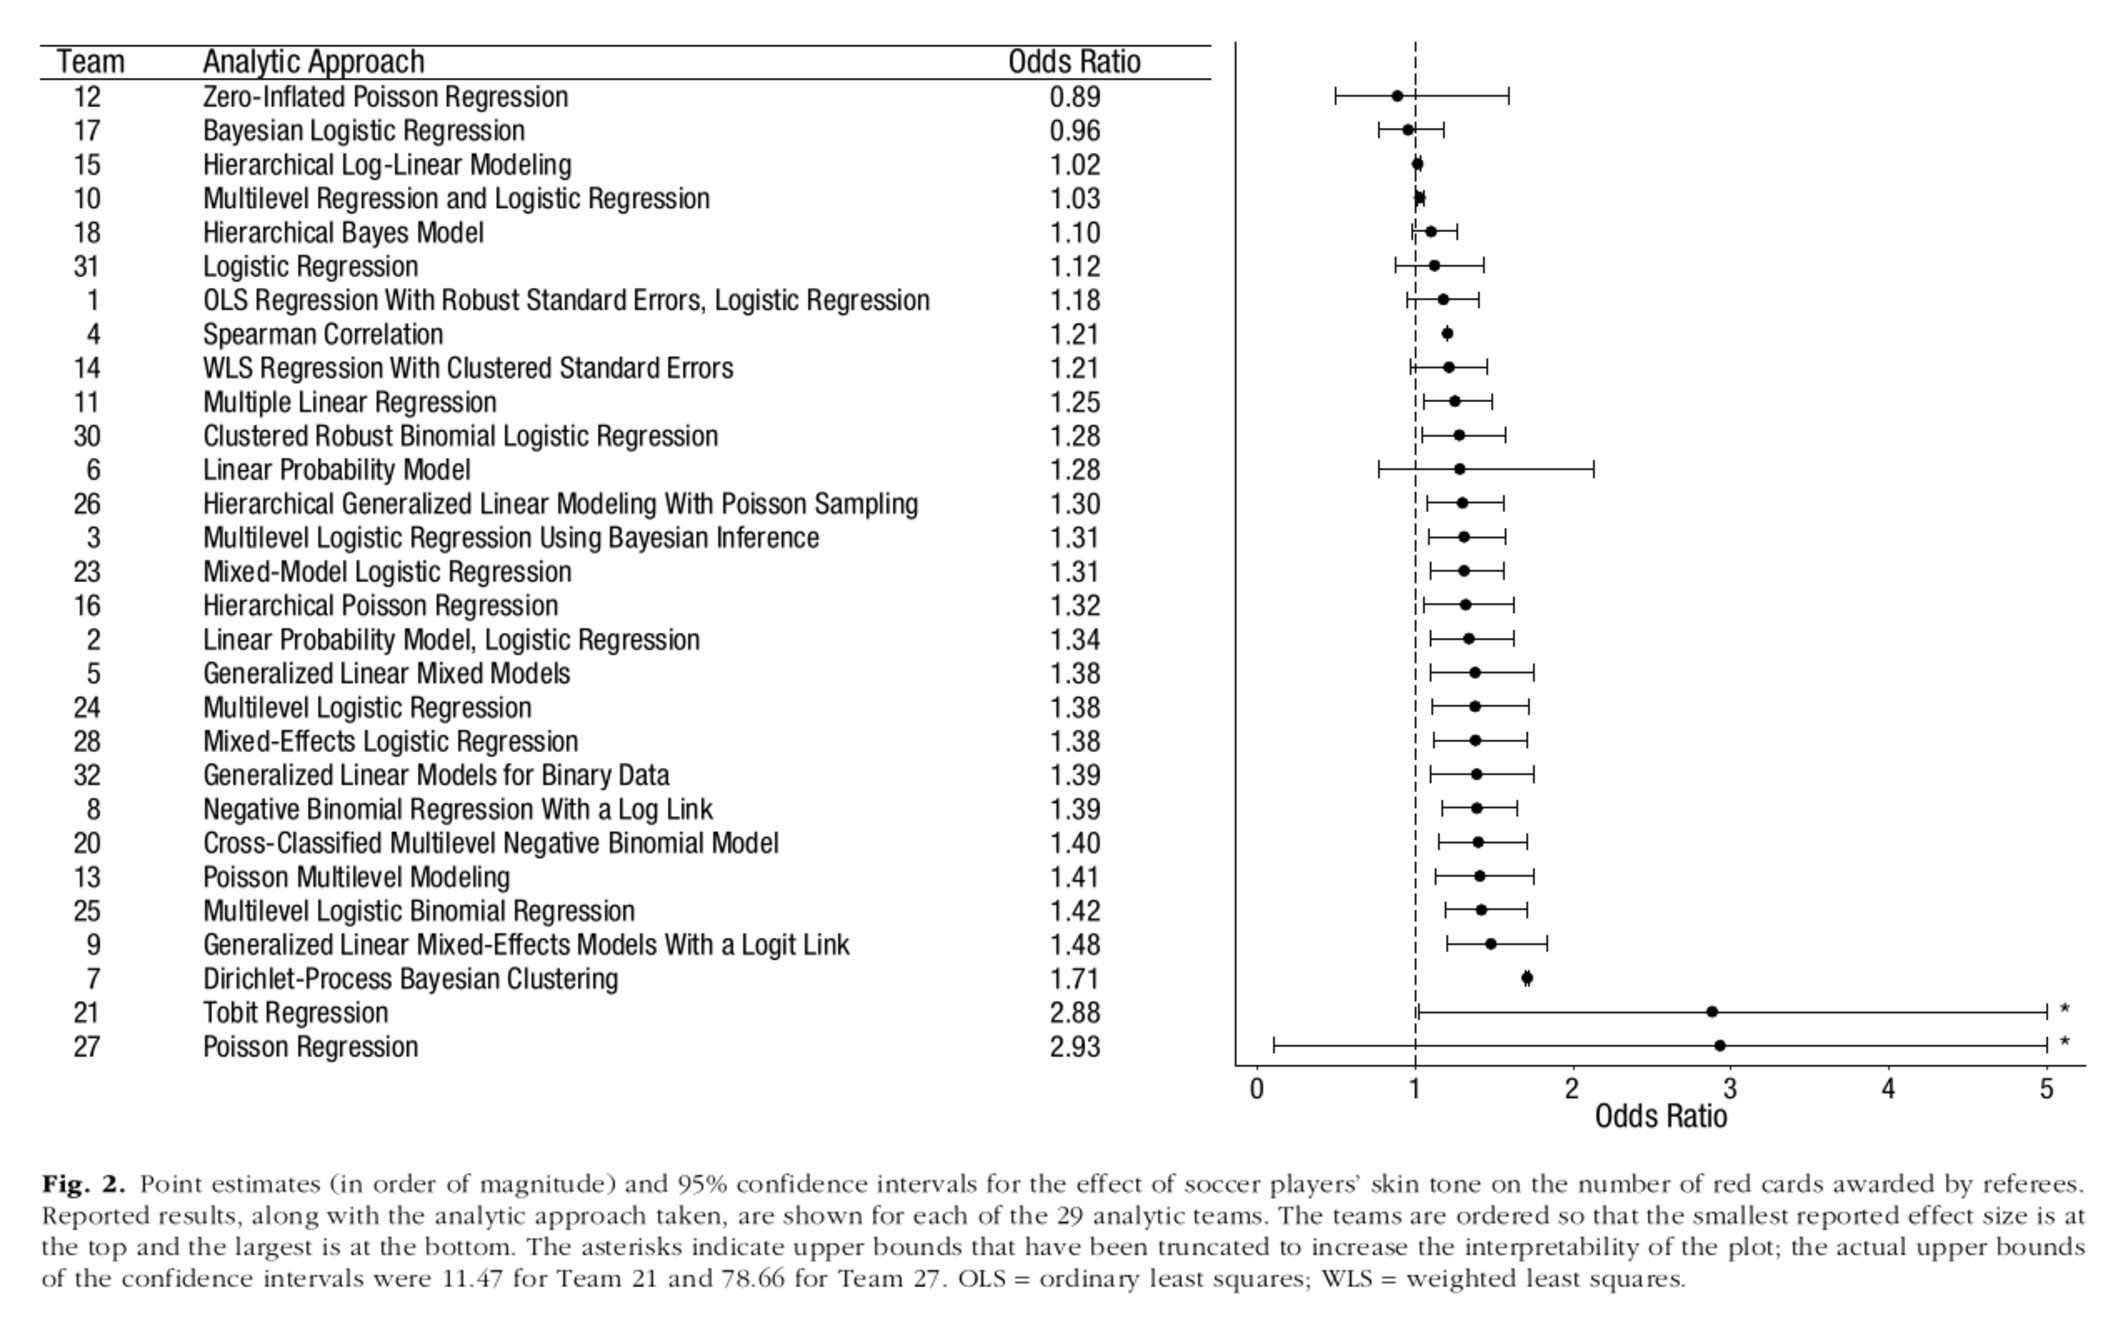
\includegraphics[scale=0.35]{silberzahn.pdf}
    \end{center}
\end{frame}

\subsection{\textit{Multiverse} analize}

\begin{frame}
    \frametitle{IV) \textit{Multiverse} analize}

    \begin{itemize}
        \item ,,A multiverse analysis starts from the observation that data used
            in an analysis are usually not just passively recorded in an
            experiment or an observational study.  Rather, data are to a certain
            extent actively constructed.''
            \bgroup
            \scriptsize
            (\citealp*[str. 702]{steegenIncreasingTransparencyMultiverse2016};
            \citealp*[za sličan pristup
            vidi][]{simonsohnSpecificationCurveDescriptive2015})
            \egroup

        \pause

        \item domisliti velik broj mogućih specifikacija problema

        \item provesti analizu uz svaku moguću specifikaciju

    \end{itemize}

\end{frame}

\begin{frame}
    \centering
    \includegraphics[scale=.25]{orben.png}

    \note[item]{N > 70000}
    \note[item]{\(\beta = -0.005\)}
    \note[item]{crveno označava \(\beta\) koje nisu statistički značajne}

    \tinycitep{orbenAssociationAdolescentWellbeing2019}
\end{frame}

\subsection{\textit{Multiverse megastudy}}

\begin{frame}
    \frametitle{\textit{Multiverse} analiza i megastudije}

    \begin{itemize}
        \item pretprocesiranje podataka
            \begin{itemize}
                \item odbaciti vremena reakcija van \(\pm 2 SD\)? \(3 SD\)?
                \item koje sudionike zadržati na temelju točnosti odgovora?
                    \(>80\%? >90\%\)?
            \end{itemize}

        \pause

        \item kako modelirati vremena reakcija?
            \begin{itemize}
                \item različiti statistički modeli

                \pause

                \item koje mjere centralne tendencije koristiti?
                    \tinycitep{rousseletReactionTimesOther2020}

                \pause

                \item kako i koju distribuciju modelirati?
                    \tinycitep{balotaMovingMeanStudies2011}

            \end{itemize}
    \end{itemize}
\end{frame}

\section{Rasprava}

\begin{noheadline}

\begin{frame}
    \sectionpage
\end{frame}

\end{noheadline}

\begin{frame}
    \begin{center}
        \begin{minipage}{25em}
            O čemu pričamo kad pričamo o procesiranju jezika?
            \tinycitep{elliottWhatTestRetestReliability2020}
        \end{minipage}
    \end{center}
\end{frame}

\begin{frame}
    \hspace*{\fill}
    \raisebox{50.5pt}{
        \begin{minipage}[t]{1em}
            \fontsize{56}{66}\selectfont
            \bfseries
            ,,
        \end{minipage}
    }
    \begin{minipage}{24em}
        The empiricist period [...] is characterized by a general
        lack of interest in stringent theoretical and metatheoretical thinking.
        [...]  Industrious research appears to be mainly driven by available
        research tools [...], methods of analysis [...], and the dynamics
        of scientific subcommunities but is surprisingly often detached from
        clearly spelled-out theories.

        \bigskip
        \scriptsize
        \raggedleft
        \citep[str. 123]{fiedlerToolsToysTruisms2004}
    \end{minipage}
    \hspace*{\fill}
\end{frame}

\begin{frame}
    \hspace*{\fill}
    \raisebox{74.5pt}{
        \begin{minipage}[t]{1em}
            \fontsize{56}{66}\selectfont
            \bfseries
            ,,
        \end{minipage}
    }
    \begin{minipage}{24em}
        There is a one-to-many mapping from scientific to statistical
        hypotheses.

        \begin{flushright}
            \bigskip
            \scriptsize
            \citep[str. 6]{gelmanGardenForkingPaths2013}
        \end{flushright}

        \bigskip

        [A] huge proportion of the verbal claims made in empirical psychology
        articles turn out to have very little relationship with statistical
        quantities they putatively draw their support from.

        \begin{flushright}
            \bigskip
            \scriptsize
            \raggedleft
            \citep[str. 2]{yarkoniGeneralizabilityCrisis2019}
        \end{flushright}
    \end{minipage}
    \hspace*{\fill}
\end{frame}

\setbeamertemplate{headline}{}

\begin{frame}[allowframebreaks]
    \frametitle{Reference}

    \bibliographystyle{apacite}
    \bibliography{../reference}
\end{frame}

\end{document}
